\documentclass[conference]{IEEEtran}

\IEEEoverridecommandlockouts

\usepackage{amsmath,amssymb,amsfonts,mathtools,bbold}
\usepackage{hyperref}
\usepackage{algorithm, algpseudocode}
\usepackage{graphicx, multirow, hhline, pgfplots}
\pgfplotsset{compat=1.18}
\usepackage{comment}

\usepackage[citestyle=numeric,bibstyle=numeric,sorting=none,maxnames=10]{biblatex}
\addbibresource{biblio.bib}
\AtBeginBibliography{\small}

\makeatletter

\newcommand{\newlineauthors}{%
\end{@IEEEauthorhalign}\hfill\mbox{}\par
\mbox{}\begin{@IEEEauthorhalign}}  

\def\hlinewd#1{%
\noalign{\ifnum0=`}\fi\hrule \@height #1 %
\futurelet\reserved@a\@xhline}

\makeatother

\begin{document}

\title{A Clustered Approach to Adaptive Kriging Particle Filter for Magnetic Field-Aided Navigation}

\author{
    \IEEEauthorblockN{Bastien HUBERT}
    \IEEEauthorblockA{\textit{DTIS, ONERA, Université Paris-Saclay} \\
    Palaiseau, France \\
    bastien.hubert@onera.fr}
\and
    \IEEEauthorblockN{Karim DAHIA}
    \IEEEauthorblockA{\textit{DTIS, ONERA, Université Paris-Saclay} \\
    Palaiseau, France \\
    karim.dahia@onera.fr}
\newlineauthors
\and
    \IEEEauthorblockN{Nicolas MERLINGE}
    \IEEEauthorblockA{\textit{DTIS, ONERA, Université Paris-Saclay} \\
    Palaiseau, France \\
    nicolas.merlinge@onera.fr}
\and
    \IEEEauthorblockN{Audrey GIREMUS}
    \IEEEauthorblockA{\textit{IMS, Université de Bordeaux, CNRS, Bordeaux INP} \\
    Talence, France \\
    audrey.giremus@u-bordeaux.fr}
}

\maketitle

\begin{abstract}
Autonomous navigation is a key aspect in unmanned mobile robotics, where accurate and efficient localisation and tracking are crucial. One of the challenges in these situations is the reliable use of sensor data, particularly in environments where GNSS is unavailable. Magnetometric navigation provides a promising alternative by leveraging the anomalies of the Earth’s magnetic field. However, accurate estimation in such settings is hindered by noises, non-linearities and scarcity of environmental information. Gaussian process regression-based particle filtering can be considered to alleviate these difficulties.

In this paper, we propose to improve Gaussian process-based particle filtering techniques by introducing a clustering step to select the relevant training data, improving their computational efficiency and accuracy in the presence of spatial non-stationarities. An auxiliary particle filter is considered due to its robustness to particle degeneracy.

The approach was validated on simulated magnetometric data for an unmanned aerial vehicle. Numerical results show that the clustering step greatly reduces the computational cost of the regression while maintaining the accuracy and convergence speed of the particle filter, demonstrating that this technique offers significant advantages for real-time autonomous navigation.
\end{abstract}

\section{Introduction}

Autonomous navigation is a fundamental challenge in aerospace robotics, particularly in scenarios where global navigation satellite system (GNSS) signals are unavailable or unreliable. In such cases, alternative methods are required to ensure accurate positioning. Magnetic field-aided navigation has emerged as a promising approach, correlating spatial variations in the Earth's magnetic field with local measurements from an embedded sensor to estimate position, as presented by \cite{bib:canciani}. However, the effectiveness of this method is limited by the inherent non-linearities in the navigation model, as well as the noisy and scarce nature of the available magnetic maps.

To address these challenges, particle filtering is commonly used instead of Kalman filters due to its ability to handle nonlinearity and multimodal probability distributions. Additionally, Gaussian process (GP) regression offers a probabilistic framework able to grasp underlying spatial dependencies and account for uncertainties, outperforming multilinear interpolation of sparse and degraded measurements.

However, using for regression all the map samples at each time step is not relevant due a prohibitive computational complexity. While \cite{bib:reduced-rank} alleviates this issue, it considers the GP to be stationary, which cannot be assumed to be the case on larger scales. As an alternative, we presented in \cite{bib:AK-RPF} an adaptive kriging method, which consisted in dynamically selecting the set of samples to be used for kriging based on their proximity with the swarm of particles. It proved efficient but failed to take into account multi-modality in the posterior probability density function to be estimated. 

In this paper, we refine the proposed approach by clustering the particles to select the relevant training data for each obtained subset of particles. By reducing the number of training points, our method significantly enhances computational efficiency while making it possible to handle spatial non-stationarity in the map and preserving estimation accuracy.

\section{Problem Statement}

Autonomous navigation situations can be formally described in a discrete state-space representation by a pair of equations: at each time step $k$, the state $x_k\in\mathbb{R}^{d_x}$ follows the dynamic $\mathcal{F}_k:\mathbb{R}^{d_x}\times\mathbb{R}^{d_\nu}\to\mathbb{R}^{d_x}$ and observes $z_k\in\mathbb{R}^{d_z}$ through the observation function $\mathcal{H}_k:\mathbb{R}^{d_x}\to\mathbb{R}^{d_z}$. Because of inaccuracies in both the dynamic and the observation models, the two equations are affected by Gaussian white noises of covariance matrices $Q_k$ and $R_k$ respectively:
\begin{equation}
\setlength\arraycolsep{1pt}
\left\{\begin{matrix*}[l]
x_k&\sim&\mathcal{N}(&\mathcal{F}_k(x_{k-1}),&Q_k&)\\
z_k&\sim&\mathcal{N}(&\mathcal{H}_k(x_k),&R_k&)
\end{matrix*}\right.\label{eq:navigation equations}
\end{equation}

Under this representation, Bayesian inference is perfectly suited to provide a state estimate by computing the posterior probability density function (PDF) of the system. The PDF can then be reduced to a single point estimator by computing its expectation:
\begin{equation}
\textstyle \hat{x}_k\triangleq\mathbb{E}(x_k|z_{1:k})=\int{x_k\:p(x_k|z_{1:k})\:dx_k}\label{eq:expectation}
\end{equation}
and its associated covariance:
\begin{equation}
\textstyle P_k\triangleq\mathbb{V}(\hat{x}_k)=\int{(x_k-\hat{x}_k)(x_k-\hat{x}_k)^Tp(x_k|z_{1:k})\:dx_k}
\end{equation}

\subsection{Particle Filter}\label{sec:PF}

While numerous techniques exist to compute the PDF using Bayesian estimation, the non-linearity and non-injectivity of the observation model makes particle filtering methods highly suited to encompass the potential multimodalities of the PDF. As presented by \cite{bib:tuto}, particle filters use importance sampling to approximate the PDF as a mixture of Dirac delta distributions:
\begin{equation}
\textstyle p(x_k|z_{1:k})\approx\sum_{i=1}^Nw_k^i\delta_{x_k^i}(x_k)
\end{equation}
where $\{x_k^i,i\in [\![1,N]\!]\}$ are the $N$ particles in $\mathbb{R}^{d_x}$ drawn at each time step according to an importance density, usually equal to the transition probability function:
\begin{equation}
x_k^i\sim q(x_k|x_{k-1}^i,z_k)=p(x_k|x_{k-1}^i)
\end{equation}

Their respective weights $w_k^i$, updated during the correction step, are expressed as follows:
\begin{equation}
w_k^i\propto w_{k-1}^ip(z_k|x_k^i)\quad\text{with}\textstyle \quad\sum_{i=1}^Nw_k^i=1
\end{equation}

The particle filter estimator corresponding to \eqref{eq:expectation} is thus the weighted sum of the particles:
\begin{equation}
\textstyle \hat{x}_k=\sum_{i=1}^Nw_k^ix_k^i
\end{equation}
and its covariance can be written as:
\begin{equation}
\textstyle P_k=\sum_{i=1}^Nw_k^i(x_k^i-\hat{x}_k)(x_k^i-\hat{x}_k)^T
\end{equation}

\subsection{Gaussian Process Regression}\label{sec:GPR}

In magnetic field-aided navigation, higher map resolutions yield better estimations. In real-world applications however, only noisy and undersampled field data is available instead of a complete map. Furthermore, because the field exhibits complex spatial dependencies, simple multilinear interpolations fail to capture its underlying intercorrelations.

A powerful alternative called kriging is presented in \cite{bib:Rasmussen}, and consists of finding the best linear unbiased estimator (BLUE) from the sampled data, provided they are realisations of the same GP. We assume that the estimation point and the samples all follow a noisy zero-mean GP:
\begin{equation}
\setlength\arraycolsep{2pt}\left\{
\begin{matrix*}[l]
&z&\sim&\mathcal{GP}(&m(x),&\mathcal{K}(x,x)+R&)\\
\forall i\in[\![1,\tilde{N}]\!],&\tilde{z}^i&\sim&\mathcal{GP}(&m(\tilde{x}^i),&\mathcal{K}(\tilde{x}^i,\tilde{x}^i)+\tilde{R}&)
\end{matrix*}\right.
\end{equation}
where $x$ and $\tilde{x}^i$ are the inputs corresponding to $z$ and $\tilde{z}^i$ respectively, $m:x\mapsto0$ is the identically zero mean of the GP, $\mathcal{K}$ is its covariance function, and $R$ and $\tilde{R}$ are the respective covariances of the additive white noises on $z$ and $\tilde{z}^i$. Using $\tilde{X}\triangleq[\tilde{x}^1\quad\cdots\quad\tilde{x}^{\tilde{N}}]$ and $\tilde{Z}\triangleq[\tilde{z}^1\quad\cdots\quad\tilde{z}^{\tilde{N}}]$, the BLUE of $z$ knowing the $\tilde{N}$ samples $\tilde{z}^i$ is:
\begin{equation}
\textstyle z^*\triangleq\sum_{i=1}^{\tilde{N}}\lambda_i\tilde{z}^i=\Lambda^T\tilde{Z}\quad\text{with}\quad\mathbb{E}(z-z^*)=0
\end{equation}
where the vector of coefficients $\Lambda$ is chosen to minimise the error covariance:
\begin{equation}
\Lambda=\text{argmin}(\mathbb{V}(z-z^*))\label{eq:minimum covariance}
\end{equation}

As proven by \cite{bib:Rasmussen}, the minimum of \eqref{eq:minimum covariance} is reached for:
\begin{equation}
z^*(x,\tilde{X},\tilde{Z})=\mathcal{K}(x,\tilde{X})\left(\mathcal{K}(\tilde{X},\tilde{X})+\tilde{R}\otimes I_{\tilde{N}}\right)^{-1}\tilde{Z}
\end{equation}
and the corresponding covariance is:
\begin{equation}
\setlength\arraycolsep{1pt}
\scalebox{0.9}{$\begin{matrix*}[l]
R^*(x,\tilde{X})=&\mathcal{K}(x,x)+R\otimes I_N-\\&\mathcal{K}(x,\tilde{X})\left(\mathcal{K}(\tilde{X},\tilde{X})+\tilde{R}\otimes I_{\tilde{N}}\right)^{-1}\mathcal{K}(\tilde{X},x)
\end{matrix*}$}
\end{equation}

\section{Clustered Adaptive Kriging Auxiliary Particle Filter (CAK-APF)}

As stated in section \ref{sec:GPR}, the available knowledge of the environment is too poor to be able to navigate with \eqref{eq:navigation equations} as is, requiring kriging of the observation function to be usable. The navigation system thus becomes:
\begin{equation}
\setlength\arraycolsep{1pt}
\left\{\begin{matrix*}[l]
x_k&\sim&\mathcal{N}\left(\vphantom{\tilde{X}}\right.&\mathcal{F}_k\left(x_{k-1}\right),&Q_k&\left.\vphantom{\tilde{X}}\right)\\
z_k&\sim&\mathcal{N}\left(\vphantom{\tilde{X}}\right.&z^*_k\left(x_k,\tilde{X},\tilde{Z}\right),&R^*_k\left(x_k,\tilde{X}\right)&\left.\vphantom{\tilde{X}}\right)
\end{matrix*}\right.\label{eq:kriged navigation}
\end{equation}

The kriged observation function requires choosing an expression for the covariance function $\mathcal{K}$, and determining its hyperparameters. Since the observation field is not supposed to be stationary, the hyperparameters cannot be determined beforehand and must be re-estimated in flight at each step of the algorithm. Furthermore, not every sample from $\tilde{X}$ is relevant depending on the spatial distribution of the particles $\{x_k^i\}$ at step $k$.

Section \ref{sec:data selection} presents an efficient method to choose the relevant samples to perform the regression, while section \ref{sec:clustering} shows how to accommodate for the non-stationarity of the field. Section \ref{sec:APF} improves particle filtering by adding a pre-propagation step, and section \ref{sec:CAK-APF} joins these components in a single algorithm.

\subsection{Data selection}\label{sec:data selection}

When choosing a covariance function $\mathcal{K}$ for the Gaussian process modelling the field, one requirement is that it must be of finite integral:
\begin{equation}
\textstyle\int\int\left|\mathcal{K}(x,\tilde{x})\right|dxd\tilde{x}<+\infty
\end{equation}

This implies that the covariance function of two inputs must tend towards $0$ as they get further away in any direction:
\begin{equation}
\mathcal{K}(x,\tilde{x})\underset{d(x,\tilde{x})\rightarrow+\infty}{\longrightarrow}0
\end{equation}

It, in turn, means that samples from $\tilde{X}$ that are too far away from any particle $x_k^i$ only add computational cost to the regression without significantly improving the estimation. To prevent this, we proposed in \cite{bib:AK-RPF} to only use samples inside a hypersphere centred around the predicted estimated state, with a radius proportional to the largest eigenvalue of the predicted covariance matrix:
\begin{equation}
S_k\triangleq\mathcal{B}\left(\hat{x}_{k|k-1},\alpha\times\underset{\lambda\in\text{sp}(P_{k|k-1})}{\text{max}}\left(3\sqrt{\lambda}\right)\right)\label{eq:data selection}
\end{equation}
where $\alpha\in[1,+\infty[$ is a dilatation coefficient, $\hat{x}_{k|k-1}$ is the predicted estimated state:
\begin{equation}
\textstyle \hat{x}_{k|k-1}\triangleq\sum_{i=1}^Nw_{k-1}^ix_k^i
\end{equation}
and $P_{k|k-1}$ is the associated predicted covariance matrix:
\begin{equation}
\textstyle P_{k|k-1}\triangleq\sum_{i=1}^Nw_{k-1}^i(x_k^i-\hat{x}_{k|k-1})(x_k^i-\hat{x}_{k|k-1})^T
\end{equation}

With this method, \eqref{eq:kriged navigation} is rewritten under its adaptive kriged form:
\begin{equation}
\scalebox{0.9}{\setlength\arraycolsep{2pt}
$\hspace*{-2mm}\left\{\begin{matrix*}[l]
x_k&\sim&\mathcal{N}\left(\vphantom{\tilde{X}}\right.&\mathcal{F}_k\left(x_{k-1}\right),&Q_k&\left.\vphantom{\tilde{X}}\right)\\
z_k&\sim&\mathcal{N}\left(\vphantom{\tilde{X}}\right.&z^*_k\left(x_k,S_k\cap\tilde{X},S_k\cap\tilde{Z}\right),&R^*_k\left(x_k,S_k\cap\tilde{X}\right)&\left.\vphantom{\tilde{X}}\right)
\end{matrix*}\right.\hspace*{-1mm}$}\label{eq:AK navigation}
\end{equation}
where $S_k\cap\tilde{Z}$ is an abuse of notation to mean "elements of $\tilde{Z}$ for which the corresponding $\tilde{x}$ are in $S_k\cap\tilde{X}$".

\subsection{Clustering}\label{sec:clustering}

Due to the spatial non-stationarity of the magnetic field, the hyperparameters of $\mathcal{K}$ cannot be assumed constant throughout space. However, particles close to each other can be assumed to share the same GP hyperparameters. For this reason, we propose to divide the particles into clusters to locally adjust the hyperparameters and perform the regression.

In this paper, we use the Mean-shift clustering algorithm, first introduced by \cite{bib:mean-shift}, as it is a non-parametric method and does not require a predefined number of clusters. It relies on kernel density estimation to find the local maxima of the PDF by gradually shifting each particle towards a maximum, and associates particles that converged to the same maximum in a single cluster. Formally, a cluster $\mathcal{C}$ is an equivalence class of the binary relation:
\begin{equation}
\left(a\equiv b\right)\quad\triangleq\quad\left(\underset{n\rightarrow+\infty}{a_n}=\underset{n\rightarrow+\infty}{b_n}\right)\label{eq:clustering}
\end{equation}
where $(x_n)_{n\in\mathbb{N}}$ is the mean-shift sequence of a point $x_0$, defined by the recursive equation:
\begin{equation}
\forall n\in\mathbb{N},x_{n+1}=m(x_n)-x_n
\end{equation}
and $m:\mathbb{R}^d\rightarrow\mathbb{R}^d$ is the weighted mean of the density given some kernel function $\kappa$:
\begin{equation}
\textstyle m:x\mapsto\sum_{i=1}^N\kappa(x^i-x)x^i\left/\sum_{i=1}^N\kappa(x^i-x)\right.
\end{equation}

Within $\mathcal{C}$, \eqref{eq:AK navigation} is modified such that \eqref{eq:data selection} becomes:
\begin{equation}
S_k^\mathcal{C}\triangleq\mathcal{B}\left(\hat{x}_{k|k-1}^\mathcal{C},\alpha\times\underset{\lambda\in\text{sp}\left(P_{k|k-1}^\mathcal{C}\right)}{\text{max}}\left(3\sqrt{\lambda}\right)\right)\label{eq:clustered selection}
\end{equation}
with $\hat{x}_{k|k-1}^\mathcal{C}$ the clustered predicted estimator:
\begin{equation}
\textstyle\hat{x}_{k|k-1}^\mathcal{C}\triangleq\sum_{x_k^i\in\mathcal{C}}w_{k-1}^{i,\mathcal{C}}x_k^i
\end{equation}
$P_{k|k-1}^\mathcal{C}$ its covariance matrix:
\begin{equation}
\hspace*{-2mm}\textstyle P_{k|k-1}^\mathcal{C}\triangleq\sum_{x_k^i\in\mathcal{C}}w_{k-1}^{i,\mathcal{C}}\left(x_k^i-\hat{x}_{k|k-1}^\mathcal{C}\right)\left(x_k^i-\hat{x}_{k|k-1}^\mathcal{C}\right)^T
\end{equation}
$\text{sp}(M)$ the spectrum of a matrix $M$, and $w_{k-1}^{i,\mathcal{C}}$ the normalised weights inside $\mathcal{C}$:
\begin{equation}
\textstyle w_{k-1}^{i,\mathcal{C}}\propto w_{k-1}^i\quad\text{with}\quad\sum_{x_k^i\in\mathcal{C}}w_{k-1}^{i,\mathcal{C}}=1
\end{equation}

\subsection{Auxiliary Particle Filter}\label{sec:APF}

While the particle filter presented in section \ref{sec:PF} is optimal for an infinite number of particles, the approximation for a finite number leads to a phenomenon of degeneracy, in which the variance of the weights of the particles increase over the iterations of the algorithm. A common solution, presented by \cite{bib:RPF}, is to add a regularisation step to the filter. However, doing so increases the variance of the particles, which is already inflated by kriging the observation function. It also introduces new parameters that can be difficult to fine-tune.

Instead, \cite{bib:APF} and \cite{bib:APF-opti} propose to model the joint probability $p(x_k,i|z_{1:k})$, where $i$ is the index of the parent particle $x_{k-1}^i$, and omitting $i$ in the estimation. The auxiliary particle filter (APF) works by choosing the importance density such that:
\begin{equation}
q(x_k,i|z_{1:k})\propto p(z_k|\mu_k^i)p(x_k|x_{k-1}^i)w_{k-1}^i\label{eq:auxiliary importance}
\end{equation}
where $\mu_k^i\sim p(x_k|x_{k-1}^i)$ are some samples, called auxiliary particles, used to assess the consistency of the parent particles with respect to the new observation $p(z_k|\mu_k^i)$. The auxiliary particles are then resampled to keep those with the highest likelihood, and their parents $x_{k-1}^{i^j}$ are used to compute the PDF.

From Bayes' theorem and using \eqref{eq:auxiliary importance}, the expressions of $\lambda_k^i$ and $w_k^j$, respectively the weights of the auxiliary and the "standard" particles can be established:
\begin{equation}
\lambda_k^i\propto p(z_k|\mu_k^i)w_{k-1}^i\label{eq:auxiliary weights}
\end{equation}
and
\begin{equation}
w_k^j\propto p\left(z_k|x_k^j\right)\left/p\left(z_k|\mu_k^{i^j}\right)\right.\label{eq:principal weights}
\end{equation}

\subsection{CAK-APF}\label{sec:CAK-APF}

Since only a kriged interpolation is available instead of the true observation function, APF needs to be adapted. While a simple way to proceed would be to add the clustering, data selection and kriging steps to two correction stages, it should be noted that $\mu_k^{i^j}$ is designed to be a good representation of the future $x_k^j$. This means that $\mu_k^{i^j}$ and $x_k^j$ are likely to belong to the same cluster, and have thus the same hyperparameters of the GP.

Algorithm \ref{alg:CAK-APF} presents the pseudo-code of CAK-APF using the same clusters and hyperparameter estimations to compute both the auxiliary and the standard weights. Notably, the clustered data selection window defined in \ref{eq:clustered selection} exclusively accounts for samples chosen by the current cluster, disregarding selections made by any other clusters.

\begin{algorithm}[ht]
\begin{algorithmic}
\For{$i\in[\![1,N]\!]$}
\State{Draw $\mu_k^i$ from $p(\cdot|x_{k-1}^i)$}\Comment{Pre-propagation}
\EndFor
\State{Compute $\left\{\mathcal{C}_k^l,l\in[\![1,c_k]\!]\right\}$ from \eqref{eq:clustering}}\Comment{Clustering}
\For{$l\in[\![1,c_k]\!]$}
\State{Compute $S_k^{\mathcal{C}_k^l}$ with \eqref{eq:clustered selection}}\Comment{Selection}
\For{$\mu_k^i\in\mathcal{C}_k^l$}
\State{Compute $z^*_k$ from clustered \eqref{eq:AK navigation}}\Comment{Kriging}
\State{Compute $\lambda_k^i$ from \eqref{eq:auxiliary weights}}\Comment{Pre-correction}
\EndFor
\EndFor
\State{$s\gets\sum_{i=1}^N\lambda_k^i$}
\For{$i\in[\![1,N]\!]$}
\State{$\lambda_k^i\gets \lambda_k^i/s$}\Comment{Normalisation}
\EndFor
\State{$\{i^j,j\in[\![1,N]\!]\}=\text{Resample}\left(\left\{\lambda_k^i,i\in[\![1,N]\!]\right\}\right)$}
\For{$j\in[\![1,N]\!]$}
\State{Draw $x_k^j$ from $p\left(\cdot|x_{k-1}^{i^j}\right)$}\Comment{Propagation}
\State{Associate $x_k^j$ to the cluster containing $\mu_k^{i^j}$}
\State{Compute $z^*_k$ from clustered \eqref{eq:AK navigation}}\Comment{Kriging}
\State{Compute $w_k^i$ from \eqref{eq:principal weights}}\Comment{Correction}
\EndFor
\State{$t\gets\sum_{j=1}^Nw_k^j$}
\For{$j\in[\![1,N]\!]$}
\State{$w_k^j\gets w_k^j/t$}\Comment{Normalisation}
\EndFor
\end{algorithmic} \caption{CAK-APF}\label{alg:CAK-APF}
\end{algorithm}

\section{Numerical Simulations for Magnetic Field Aided Navigation}

\subsection{Application to Magnetic Field Aided Navigation}

The use case chosen in this paper to illustrate CAK-APF is an unmanned aerial vehicle (UAV) flying in a rectilinear uniform motion over Mexico, as shown by figure \ref{fig:trajectory}.

\begin{figure}[ht]
\centerline{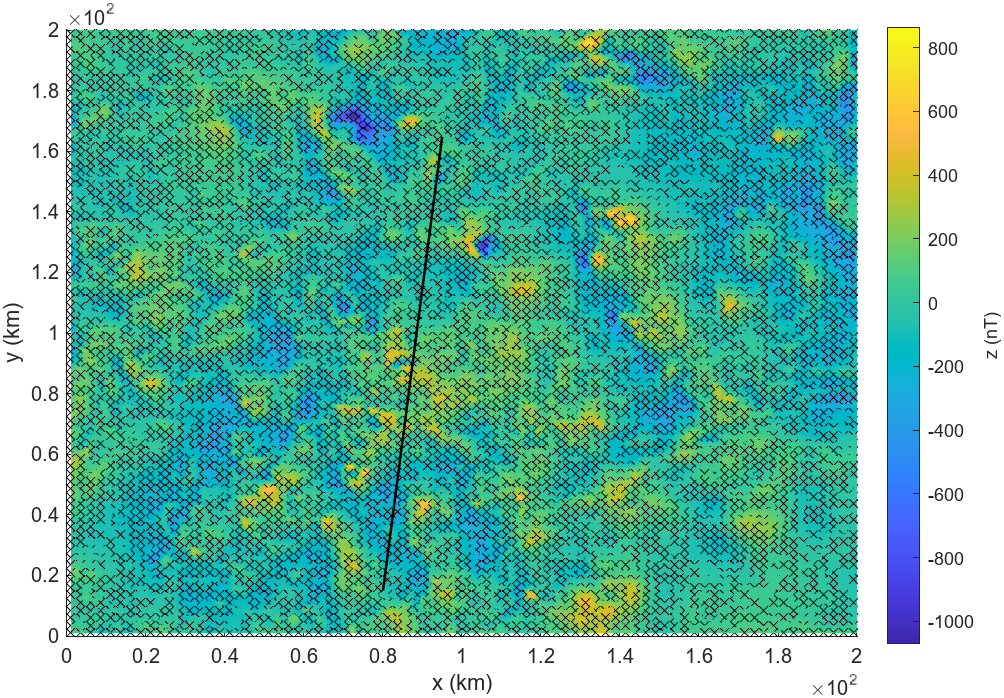
\includegraphics[width=0.4\textwidth]{../../Images/MAG_trajectoire.png}}
\caption{Trajectory of the UAV over Mexico's magnetic anomaly field} \label{fig:trajectory}
\vspace{-\baselineskip}
\end{figure}

The UAV observes the sampled data $\tilde{X}$, symbolised by the $\times$ markers, of the local magnetic anomaly field, the data for which comes from \cite{bib:carte-magnétique}. Its state is fully described by the $d_x=4$ dimension vector $x=\begin{bmatrix}p_x&p_y&v_x&v_y\end{bmatrix}^T$, with $p_x$ and $p_y$ being the x and y coordinates of the UAV, and $v_x$ and $v_y$ their respective velocities. The dynamical model of the UAV is given by:
\begin{equation}
\mathcal{F}_k:x\in\mathbb{R}^4\mapsto\begin{bmatrix}I_2&\Delta_tI_2\\0&I_2\end{bmatrix}x
\end{equation}
where $\Delta_t$ is the sampling period of the algorithm, and $I_2$ is the identity matrix of size $2$.

In order to evaluate the different steps of CAK-APF, simulations were performed on four different filters:
\begin{itemize}
\item The standard APF with known map instead of kriging;
\item A static kriging APF, using every samples to perform the regression (the estimation of the hyperparameters is done once before the start of the Monte-Carlo runs);
\item An adaptive kriged APF without clustering;
\item CAK-APF as presented by algorithm \ref{alg:CAK-APF}.
\end{itemize}

$N_{MC}$ Monte-Carlo runs are performed per filter, during which an estimation of the state $\hat{x}_k$ is iteratively computed over $N_{iter}$ iterations from an unknown state drawn from a Gaussian distribution centred around the true initial state $x_0$, with covariance $P_0$. Table \ref{tab:parameters} gives the values of the chosen parameters.
\begin{table}[ht]
\renewcommand{\arraystretch}{1.1}
\centering \caption{Simulation and CAK-APF parameters} \label{tab:parameters}
\begin{tabular}{r|l}\hline
Parameters&Value\\\hline
$N_{MC}$&$100$\\
$N_{iter}$&$600$\\
$\Delta_t$&$0.5\text{s}$\\
map surface&$200\text{km}\times200\text{km}$\\
map resolution&$1\text{km}\times1\text{km}$\\
$P_0$&$\text{diag}([3000\text{m},3000\text{m},3\text{m.s}^{-1},3\text{m.s}^{-1}])^2$\\
$N$&$5000$\\
$Q_k$&$\text{diag}([40\text{m},40\text{m},0.4\text{m.s}^{-1},0.4\text{m.s}^{-1}])^2$\\
$R_k$&$80^2\text{ nT}^2$\\
$\tilde{N}$&$80^2$\\
$\tilde R$&$80^2\text{ nT}^2$\\
$\alpha$&$2$\\
resampling algorithm&Kitagawa resampling from \cite{bib:tuto}\\
$\kappa$&Gaussian kernel from \cite{bib:Rasmussen}\\
hyperparameter estimation&likelihood gradient ascent from \cite{bib:Rasmussen}\\
$\mathcal{K}$&Epanechnikov function from \cite{bib:Rasmussen}\\\hline
\end{tabular}
\end{table}

\subsection{Numerical Results}

For each filter, their root mean square error (RMSE) has been calculated according to:
\begin{equation}
\text{RMSE}:k\in[\![1,N_{iter}]\!]\mapsto\sqrt{\frac{\sum_{m=1}^{N_{MC}}||\varphi(x_k-\hat{x}_{k,m})||_2^2}{N_{MC}}}
\end{equation}
where $\varphi:\begin{bmatrix}p_x&p_y&v_x&v_y\end{bmatrix}^T\mapsto\begin{bmatrix}p_x&p_y\end{bmatrix}^T$ is the projector on the positions, $x_k$ is the true state at time $k$, and $\hat{x}_{k,m}$ is the corresponding estimation by the $m$-th Monte-Carlo run. A histogram of the number of the samples used to perform the kriging step for each filter has also been computed. Figure \ref{fig:RMSE} gives the RMSEs over time of the four filters, and figure \ref{fig:histogram} presents their corresponding histogram.

\begin{figure}[ht]
\centerline{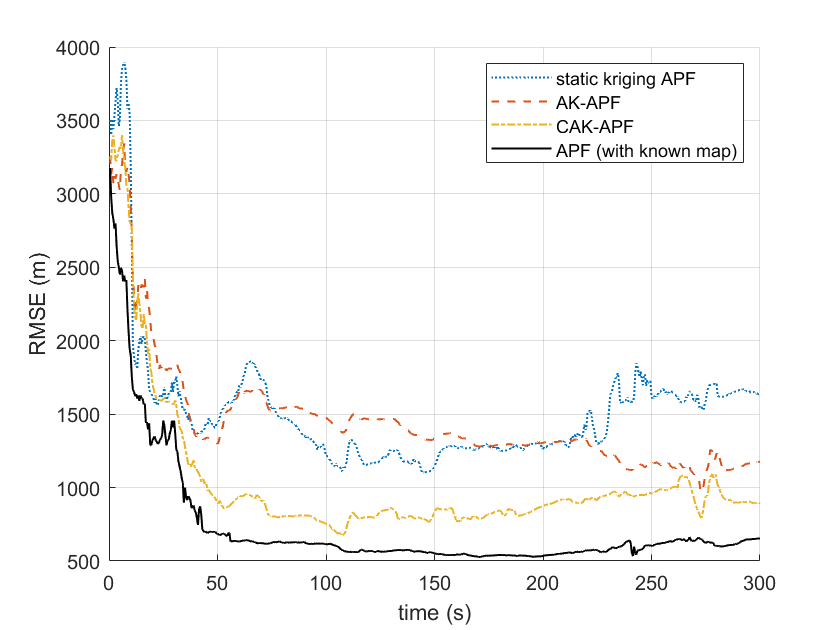
\includegraphics[width=0.4\textwidth]{../../Images/RMSE.png}}
\caption{RMSE over time of the tested filters} \label{fig:RMSE}
\end{figure}

\begin{figure}[ht]
\centerline{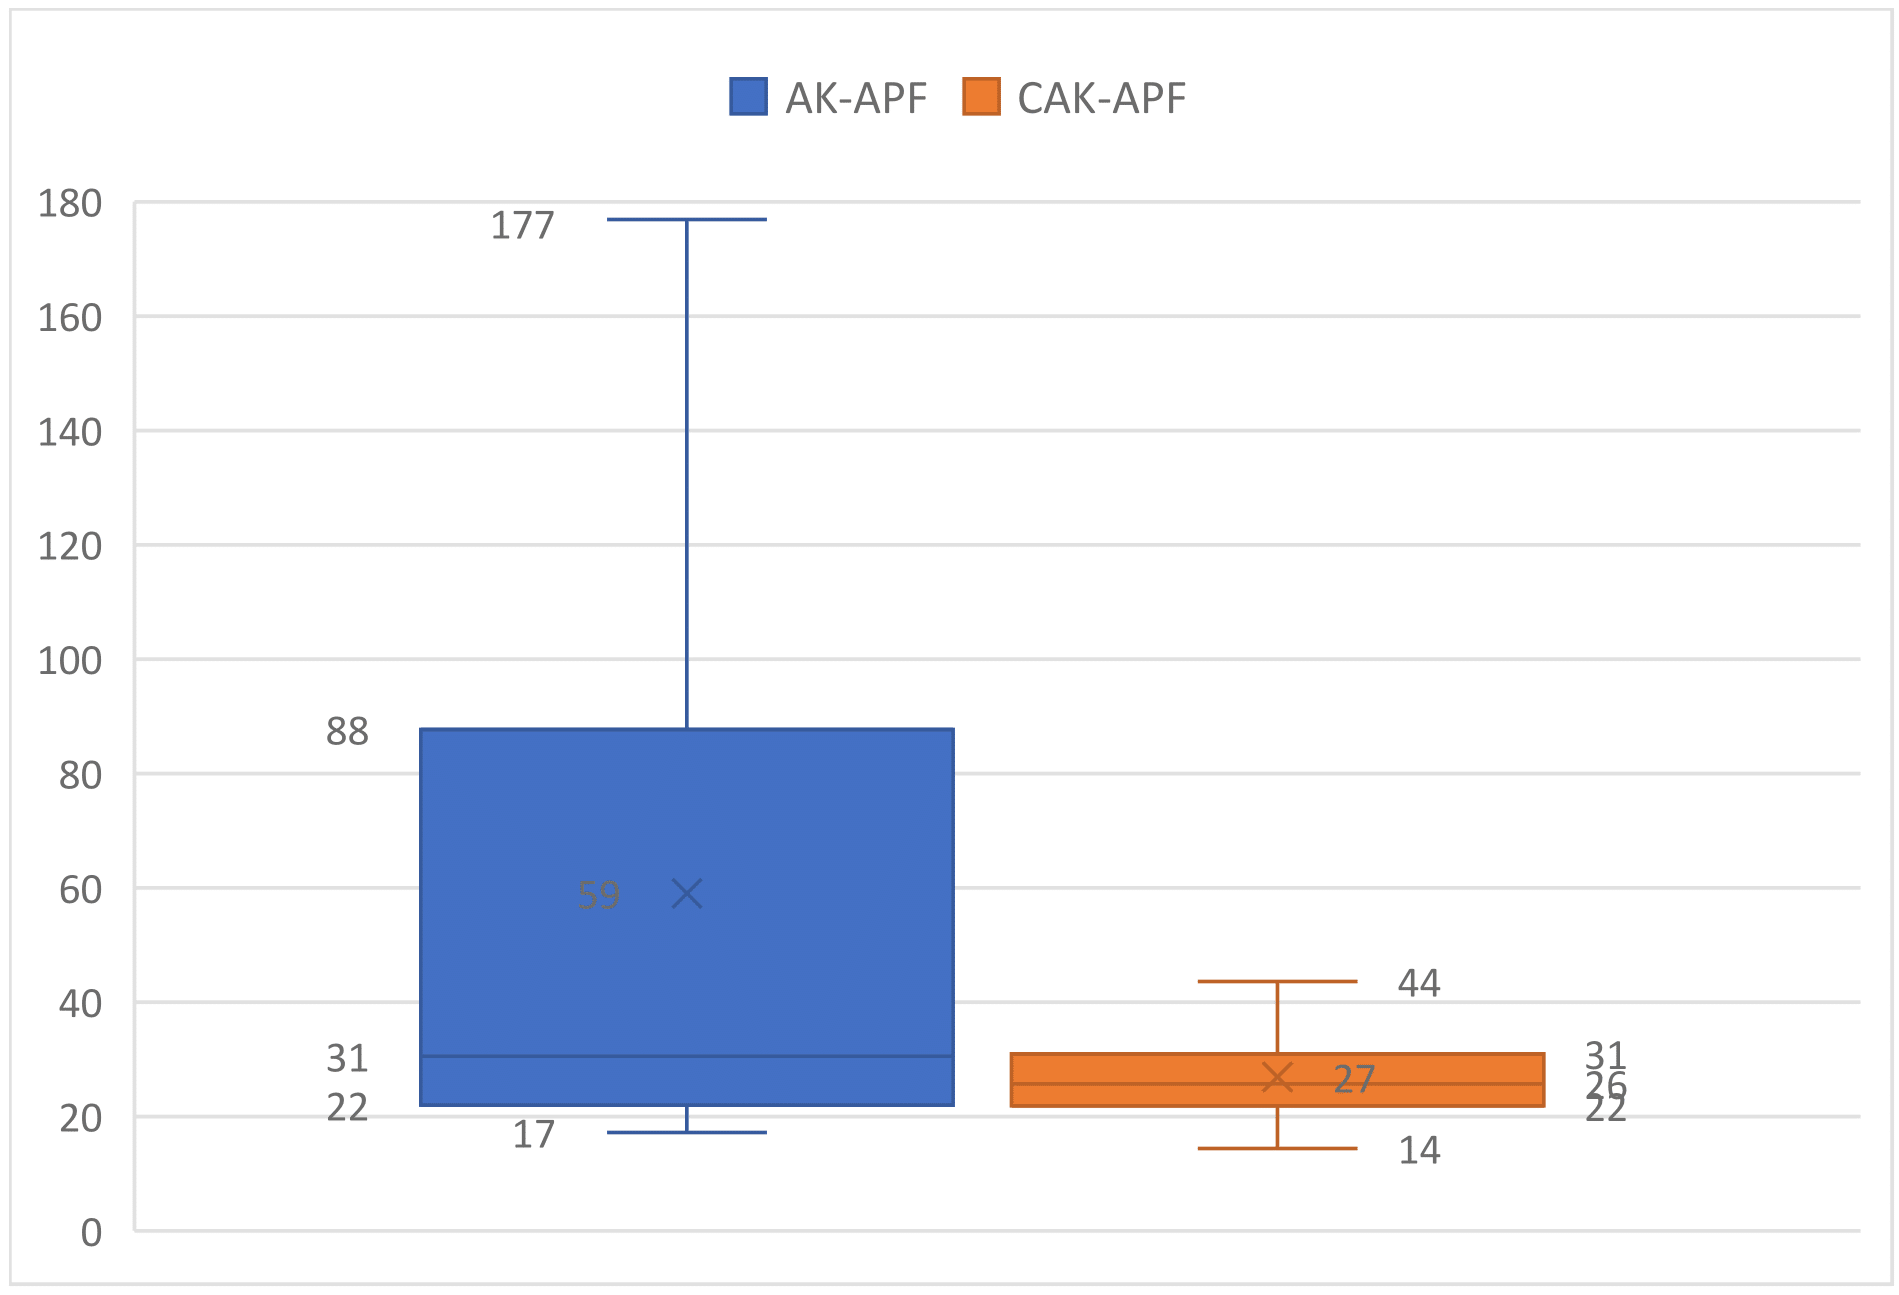
\includegraphics[width=0.4\textwidth]{../../Images/histogrammes.png}}
\caption{Histogram of the number of selected sampled used in the tested filters} \label{fig:histogram}
\vspace{-\baselineskip}
\end{figure}

Unsurprisingly, the greatest accuracy is achieved when APF has access to the full and undisturbed map. On the other hand, it must be noted that reconstructing the whole map with a static Gaussian process prior to navigation yields mitigated results. This can be explained by the non-stationarity of the anomaly field, whose hyperparameters seem to have been adequately estimated for iterations $75$ to $200$, but are less representative outside this range. Similarly, while performing better than its static counterpart, AK-APF exhibits a wide spread in the selected samples, as determined by the covariance matrix from \eqref{eq:data selection}. This results in a slower convergence and prevents it from reaching the sub-kilometre accuracy of CAK-APF.

While figure \ref{fig:histogram} shows that the median numbers of samples for the adaptive kriging methods are relatively close, the upper part of the distribution is much larger for AK-APF than for CAK-APF. This is caused by highly multimodal situations, where AK-APF encompasses irrelevant samples between clusters, in areas where there are no particles. On the other hand, the much narrower distribution of CAK-APF ensures a more consistent computation time, which is crucial in real-time applications.

For $N$ particles, $\tilde{N}$ samples, and $T<<N$ iterations required by Mean-shift to converge, the complexities of Mean-shift, data selection and hyperparameter learning, and kriging are $\mathcal{O}(TN^2)$, $\mathcal{O}(\tilde{N}^3)$, and $\mathcal{O}(N\tilde{N}^2)$ respectively. For an average of $2$ clusters, $T\approx15$, and considering that CAK-APF uses on average $46\%$ less samples than its AK counterpart, this means that CAK is more than $2.5$ faster than AK on average, both of which are more than $6$ orders of magnitude faster than static kriging. The gap is even wider considering that the histogram counts the selected data from every cluster of a single iteration, so only a fraction of the samples is simultaneously used, further decreasing the computational cost of CAK-APF.

\section{Conclusion and Perspectives}

In this paper, we improved GP-based particle filtering by introducing a clustering step to select the most relevant training data for the kriging step. By locally estimating the hyperparameters of the GP modelling the environment, we increased both computational speed and accuracy. Through simulations of a UAV navigating with magnetic anomaly data, we showed significant improvements from both static kriging and a simpler adaptive algorithm from which this version is based.

The results show that clustering particles not only optimises the use of available samples but also ensures that the non-stationarity of the magnetic field is adequately addressed. CAK outperformed its counterparts, offering an effective solution for real-time autonomous navigation in environments where global navigation satellite systems are unavailable or unreliable. Furthermore, the use of  APF helped mitigating the particle degeneracy problem without introducing additional parameters, thus enhancing the robustness of the algorithm.

Future work will focus on exploring other methods for data selection and computing formal error bounds for the approximated observation model. Additionally, incorporating real-time adaptation of the magnetic field model and introducing a simultaneous localisation and mapping (SLAM) formalism could provide insights into its performance and scalability in operational environments.

\printbibliography

\end{document}
